% !TeX spellcheck = en_GB
% !TeX encoding = UTF-8

% COMPILE WITH:
% `latexmk`
% You need lualatex and biber (in all TeXLive distributions)
\documentclass[
numbers=noenddot,
%listof=totoc,
parskip=half-,
fontsize=12pt,
paper=a4,
oneside,
titlepage,
bibliography=totoc,
chapterprefix=false,
table
%    draft
]{scrbook}

%\usepackage[utf8]{inputenc}
%\usepackage[T1]{fontenc}
\usepackage[ngerman]{babel}
\usepackage{algorithmicx}
\usepackage{algorithm}
\usepackage{algpseudocode}
\usepackage{graphicx}
\usepackage{array}
\usepackage{amsmath}
\usepackage{pdflscape}


%pgfplots
\usepackage{pgfplots}
\pgfplotsset{width=10cm,compat=1.9} 
\usepgfplotslibrary{external}
\tikzexternalize 

% use lualatex or xelatex
%\usepackage{fontspec}
\usepackage{wrapfig}
\usepackage[onehalfspacing]{setspace}

% better language support
\usepackage{polyglossia}
\setdefaultlanguage{english}
%\setdefaultlanguage{german}

\usepackage{tocbasic}
\usepackage{booktabs}
\usepackage{multicol}
\usepackage{multirow}
\usepackage{paralist}
\usepackage[]{scrlayer-scrpage}

% better bibliography (biblatex style)
% use biber to compile
\usepackage[citestyle=alphabetic, bibstyle=alphabetic, sorting=nyt, backend=biber, language=english, backref=true, maxcitenames=2]{biblatex}

% better quotes
% use \enquote{text}
\usepackage[autostyle,english=american,german=quotes]{csquotes}
\addbibresource{bibliography.bib}

% appendix
\usepackage[titletoc]{appendix}
\usepackage[T1]{fontenc}
\usepackage{siunitx}
\usepackage{float}
\usepackage[utf8]{inputenc}
\usepackage{hyperref}
\usepackage{subfiles}
\usepackage{subfig}
%\usepackage[table]{xcolor}

% where to put all images and figures
\graphicspath{{images/}}

% Title
\title{Scratch Bug Detection Using the N-gram Language Model}

% Author
\author{Eva Gründinger}

% Date
\date{\today}

% CHOOSE ACCORDINGLY
\newcommand{\thesisType}{bachelor's thesis}
%\newcommand{\thesisType}{Masterarbeit}

\makeatletter
\let\thetitle\@title
\let\theauthor\@author
\let\thedate\@date
\makeatother

\pagestyle{scrheadings}

\begin{document}

%%%%%%%%%%%%%%%%%%%%%%%%%%%%%%%%%%%%%%%%%%%%%%%%%%%%%%%%%%%%%%%%%%%%%%%%%%%%%%%%%%%%%%%%%
\frontmatter
% CHOOSE ACCORDINGLY
% !TeX spellcheck = de_DE
% !TeX encoding = UTF-8
% !TeX root = ../thesis.tex
\begin{titlepage}
    \centering
    \begin{onehalfspace}
    
        	
\includegraphics[width=7cm]{uni-logo.png}\\
        	\vspace{1.0cm}
        	\large {\bfseries Chair of Software Engineering II} \\

        	\vspace{2.5cm}

            \begin{doublespace}
            	{\textsf{\Huge{\thetitle}}}
            \end{doublespace}

        	\vspace{2cm}

            \Large{Bachelor Thesis by}\\

        	\vspace{1cm}

        	{\bfseries \large{\theauthor}}

        	\vfill

        	{\large
        		\begin{tabular}[l]{cc}
        			\textsc{Advisor}\\
        			Prof.~Dr.~Gordon Fraser
        		\end{tabular}
        	}

        	\vspace{1.5cm}

        	\parbox{\linewidth}{\hrule\strut}

            \vfill

	    {\thedate}
    	
    \end{onehalfspace}
\end{titlepage}

%\include{includes/MA-titlepage}

\phantomsection
\addcontentsline{toc}{chapter}{Contents}
\tableofcontents
\newpage




% -- ABSTRACT
\newcommand{\ngram}{\textsc{n-gram language model}}
\newcommand{\litterbox}{\textsc{LitterBox}}
\newcommand{\scratch}{\textsc{Scratch}}
\newcommand{\bugram}{\textsc{Bugram}}
\newcommand{\java}{\textsc{Java}}
\newcommand{\latex}{\textsc{LaTex}}
\newcommand{\hairball}{\textsc{Hairball}}
\newcommand{\drscratch}{\textsc{Dr. Scratch}}
\newcommand{\whisker}{\textsc{Whisker}}
\newcommand{\AST}{\textsc{AST}}

\newtheorem{definition}{Definition}

\phantomsection
\addcontentsline{toc}{chapter}{Abstract}
% !TeX spellcheck = en_GB
% !TeX encoding = UTF-8
% !TeX root = ../thesis.tex
\chapter*{Abstract}
%TODO Unfinished chapter!

In contrast to rule-based methods which often rely on special patterns that appear rather frequently in source code, and detect violations based on the inferred rules, the \ngram{} is another approach to bug detection. In this bachelor's thesis, this new way of software bug detection is proposed in order to improve software reliability and the quality of \scratch{} programs.

After the tokenization, token sequences are assessed with their calculated probabilities which are based on the existing model. If a detected token sequence has a rather low probability, it gets reported as a potential bug because the assumption is that these kinds of sequential tokens are unusual and should be highlighted to the programmer as a bad practice or programming mistake that affects the program.

The \ngram{} gets evaluated in the following ways. First, \scratch{} projects are analysed to find bugs, code smells or unusual use cases. Then the result is compared to the reported bugs by \litterbox{} which assesses the same projects. The \ngram\ reported sequences for each task although \whisker\ tests may have passed and no code smells were found by \litterbox{} which shows the different kind of violations n-gram models are able to detect.

Second, detected bugs are categorized to identify if \ngram{s} are suitable for bug detection in \scratch{} projects and if this implementation is able to compete with already existing approaches like \litterbox{}. The project-specific \ngram\ can detect extensions to an original task, which \litterbox\ is not able to do, as well as dead code and empty scripts/bodies, whereas unused variables or long scripts are not in its reported violations.  

Third, it is analysed if the \ngram\ is able to get valid results with a set of tasks that were openly completed. The analysis demonstrates that this approach of bug detection is even effective in circumstances where solutions of tasks are only fairly related to each other. The project-specific model is still able to identify potential bugs with the exception of the possibility to categorize unusual use cases due to missing reference solutions.

Fourth, a comparison between a general \ngram\ and project-specific models showed that the general model out of a big data set is not as useful than project-specific ones. For instance, unusual use cases cannot be detected because of missing reference solutions. To have exact numbers that demonstrate the accuracy of the estimations, further research is needed to give the calculated negative probabilities more meaning. 

The results suggest that the implementation this bachelor's thesis is referring to is complementary to the above mentioned methods of software analysis.


\newpage

% -- Acknowledgements (optional)
%% !TeX spellcheck = en_US
% !TeX encoding = UTF-8
\chapter*{Acknowledgments}

% I would first like to thank my thesis advisor ...
\newpage

\phantomsection
\addcontentsline{toc}{chapter}{List of Figures}
% -- List of figures
\thispagestyle{empty}
\cleardoublepage
\listoffigures
\newpage

%% -- List of algorithms
%\thispagestyle{empty}
%\cleardoublepage
%%\listofalgorithms
%\newpage

\phantomsection
\addcontentsline{toc}{chapter}{List of Tables}
% -- List of tables
\thispagestyle{empty}
\cleardoublepage
\listoftables

\newpage

%%%%%%%%%%%%%%%%%%%%%%%%%%%%%%%%%%%%%%%%%%%%%%%%%%%%%%%%%%%%%%%%%%%%%%%%%%%%%%%%%%%%%%%%%
\mainmatter

% -- Chapters
% following IMRaD structure
% adjust for your liking
% !TeX spellcheck = en_GB
% !TeX encoding = UTF-8
% !TeX root = ../thesis.tex
\chapter{Introduction}\label{chap:introduction}
%TODO !F: Unfinished chapter! (Check example probabilities)

As one of the most popular block-based programming languages \scratch{}~\cite{scratch} has established a growing community over the years that surrounds a database of almost 60 million created projects\footnote{\url{https://scratch.mit.edu/statistics/}, last accessed September 01, 2020}. Because of the fun and easy programming environment that supports novice programmers particularly in their creative process, \scratch{} is preferred by students over text-based languages when it comes to studying about the world of programming. The drag-and-drop principle of puzzle pieces helps beginners to avoid common syntax mistakes and encourages children in a fun way to take control over the \textit{stages} and \textit{sprites} and create their own world and stories. Memorization instead of recall is an important part of the \scratch{} system because by picking your favourite blocks from a palette instead of having to know all commands right away is helping programming novices to get fast and viewable results. 

Though \scratch{} makes programming seem easy, there are also many mistakes that programmers can commit if they are unaware of common programming practices. The frustration of finding these bugs in a huge number of code blocks is even more apparent as a teacher who has to examine each project manually because of missing tools in the \scratch{} editor that usually are a part of every standard programming frameworks, like Intellij\footnote{\url{https://www.jetbrains.com/idea/}, last accessed September 01, 2020} or Eclipse\footnote{\url{https://www.eclipse.org/}, last accessed September 01, 2020}. In order to support \scratch{} users and improve their code quality and accuracy, there are many researchers who find methods to detect bug patterns~\cite{scratch_bugpatterns} as well as code smells~\cite{badsmells, badhabits, hairball} or even implemented automated approaches for testing~\cite{whisker} for the \scratch{} environment. As a result, tools like \hairball~\cite{hairball}, \drscratch~\cite{drscratch} or \litterbox~\cite{scratch_bugpatterns} were created to further the analysis of \scratch{} programs and assist programmers in their bug detection process.

In order to improve code quality and reliability of programs, many rule-based techniques have been researched to detect bugs and code smells. However, these rule-based approaches are relying on highly frequent patterns in the code. Another approach is the usage of \ngram{s} for code analysis. This way of detecting defective code is already successfully applied by \bugram{}~\cite{bugram} on \java{} code. The assumption is that low probability token sequences are unusual, which may indicate bugs, bad practices or special uses of code. 

The \ngram{} works by assessing token sequences of programs by their probability in the learned model while low probability ones are marked as bugs. For bug detection the five main components that need to be configured for the model are: \textit{Gram size, sequence length, reporting size, maximum probability threshold} and \textit{minimum token occurrence}. After adjusting these settings, the n-gram Markov model is able to obtain the probabilities of all token sequences. The probability of each token in a sequence is only determined by its previous n-1 tokens. Using a 3-gram model the probability of the sequence s is calculated like it is shown in the Equation~\ref{eq:sequence_prob}. Then the language model ranks the outcome based on its probability in descending order and reports the sequences with the lowest probabilities as potential bugs. 
 
\begin{equation} \label{eq:sequence_prob}
P(s) ={} P(b_{1})\cdot P(b_{2}\mid b_{1})\cdot P(b_{3}\mid b_{1}b_{2})\cdot P(b_{4}\mid b_{2}b_{3})
\end{equation}

\begin{figure}%
    \centering
    \subfloat[First script of monkey sprite]{{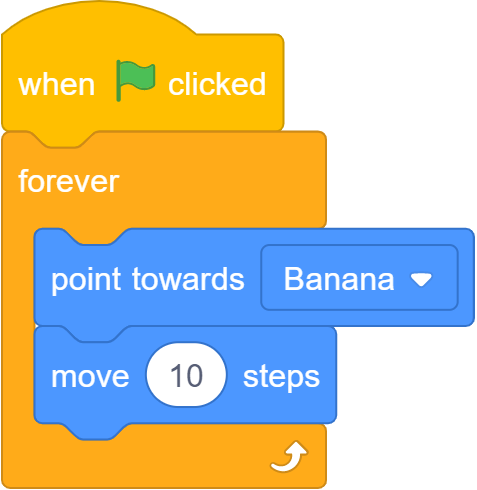
\includegraphics[width=5cm]{exampleTokens(1).png}\label{fig:exampleTokens(1)} }}%
    \qquad
    \subfloat[Second script of monkey sprite]{{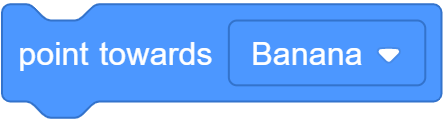
\includegraphics[width=5cm]{exampleTokens(2).png}\label{fig:exampleTokens(2)} }}%
    \caption[Example bug detection with \ngram{}]{\label{fig:exampleTokens}Example bug detection with \ngram{}}%
\end{figure}

In this bachelor's thesis a technique that uses \ngram{s} to automatically detect bugs in \scratch{} programs is proposed. For instance, Figure~\ref{fig:exampleTokens} shows \scratch\ scripts that were created as a solution for the monkey task and control the monkey sprite in the project. 

The block sequence [Never, GoToPos], shown in Subfigure~\ref{fig:exampleTokens(2)}, can basically never be executed because of a missing \textit{hat block}. Consequently, it is a rather unusual sequence and has only a probability of 0.12\%, whereas the sequence [GreenFlag, RepeatForeverStmt], which can be found as the first two blocks in Subfigure~\ref{fig:exampleTokens(1)}, is a common use case with an occurrence probability of 7.18\%. Therefore, the sequence [Never, GoToPos] is suspicious and indicates the existence of a code smell or bug. 

This is an example of how to use the \ngram\ to find low probability sequences and mark them as potential bugs that should be further analysed by the programmer. The accuracy of the probability calculation depends on many configuration parameters of the model and calculation methods like \textit{Smoothing} that will be further explained in this bachelor's thesis. 

% !TeX spellcheck = en_GB
% !TeX encoding = UTF-8
% !TeX root = ../thesis.tex
\chapter{Background}\label{chap:background}
As this thesis merges known concepts from \scratch{} analysis and \ngram{}, we introduce the concepts our work is based on in the following sections. Section~\ref{sec:analysing-scratch} introduces \scratch{} and its functionality as a block-based programming language as well as the \scratch{} analyser \litterbox{}. Section~\ref{sec:language-models} introduces the concept of a \ngram{}. It is necessary to understand the difference between n-grams and a n-gram model and the way of using it in order to obtain valuable information about \scratch{} code.


\section{Analysing \scratch{} Programs}\label{sec:analysing-scratch}

% \textit{blocks}\footnote{\url{https://en.scratch-wiki.info/wiki/Blocks}, last accessed April 29, 2020}
% \hyperref[def:code-smells]{code smells}
\subsection{The Structure of \scratch{}}\label{subsec:scratch}
\scratch{}\footnote{\url{https://en.scratch-wiki.info/wiki/Scratch}, last accessed August 19, 2020} is a block-based programming language designed for kids that was created by the Massachusetts Institute of Technology (MIT). With over 50 million registered users and shared projects\footnote{\url{https://scratch.mit.edu/statistics/}, last accessed August 19, 2020} it is one of the most popular tools for teaching children from a young age how to develop computational thinking skills to solve problems programmatically.

The 'drag-and-drop-programming' style that \scratch{} is utilizing allows the programmer to pick from a pallet of existing blocks and build scripts by combining these code pieces like a jigsaw puzzle.
\textit{Blocks}\footnote{\url{https://en.scratch-wiki.info/wiki/Blocks}, last accessed August 19, 2020} are separated into different types that include \textit{hat, stack, reporter, boolean and cap}. Each data type has a specific shape that indicates their intended usage in order to avoid errors in the syntax of the code. In contrast to text-based programming languages, the \textit{blocks} help children to memorize the commands and avoid structure errors that otherwise would very likely occur in the beginning. 

After combining different \textit{blocks}, \textit{scripts}\footnote{\url{https://en.scratch-wiki.info/wiki/Script}, last accessed August 19, 2020} are created which resemble code methods in \java{}. \textit{Scripts} are found in the code of the actors that perform the actions, called \textit{sprites}\footnote{\url{https://en.scratch-wiki.info/wiki/Sprite}, last accessed August 19, 2020} as well as the \textit{stage}\footnote{\url{https://en.scratch-wiki.info/wiki/Stage}, last accessed August 19, 2020} which visualises the background of the created program. 

% TODO Add example code (script with picture)

\subsection{The Static \scratch{} Code Analyser \litterbox{}}\label{subsec:litterbox}
\litterbox{}\footnote{\url{https://gitlab.infosun.fim.uni-passau.de/se2/litterbox}, last accessed August 19, 2020} is a static code analysis tool for detecting bugs in \scratch{} projects. The occurrence of bugs in code is mostly the consequence of recurring bad code writing habits that visualise in code smells and refactoring opportunities. With the help of \litterbox{} these bug patterns can be filtered and analysed in order to fix found bugs and avoid similar mistakes in the future. \litterbox{} is developed at the Chair of Software Engineering II and the Didactics of Informatics of the University of Passau.

% TODO Add access information for LitterBox


\section{N-gram Language Model}\label{sec:language-models}
% TODO Introduce language models

\subsection{Definition of N-grams}\label{subsec:ngram}
% TODO Explain Markov chain and probability calculation

\subsection{Probability Calculation with N-gram Model}\label{subsec:ngram}
% TODO Define key words (Token, GramSize, SequenceLength, ReportingSize, Minimum Token Occurence, Probability Threshold






% !TeX spellcheck = en_GB
% !TeX encoding = UTF-8
% !TeX root = ../thesis.tex
\chapter{N-gram Bug Detection in \scratch{}}\label{chap:methods}

\begin{figure}[hbtp]
\centering
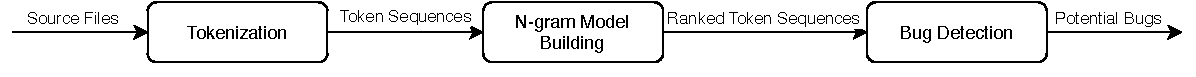
\includegraphics[scale=0.75]{images/Overview.pdf}
\caption{Overview of the N-gram model building process}
\label{fig:overview}
\end{figure}

Figure \ref{fig:overview} visualises the \ngram{} building process which is explained in this chapter in more detail. In Section~\ref{sec:tokenization} the tokenization process is described with the way the \scratch{} project is parsed and converted into tokens. The next step is to use the created tokens to build the \ngram{} like it is shown in Section~\ref{sec:model}. Finally, bugs can be detected with the help of the calculated model according to Section~\ref{sec:detection}.

\section{Tokenization of \scratch{} Code}\label{sec:tokenization}
In order to build a model, we need to tokenize the \scratch{} project into suitable pieces:

\begin{definition}[Token]\label{def:token}
    %
    ``A token is a single fragment of \scratch{} code that is used to partition code into smaller pieces in order to obtain information about its syntax on a specific granularity level.''
    %
\end{definition}

In order to identify unusual block sequences in a \scratch{} project, each project should be represented in the same form and structure. To visualise a \scratch{} project like it is shown in Figure~\ref{fig:ast}, the tokenization process is based on the abstract syntax tree (\AST{}) structure of \litterbox{}. 

\begin{figure}[hbtp]
\centering
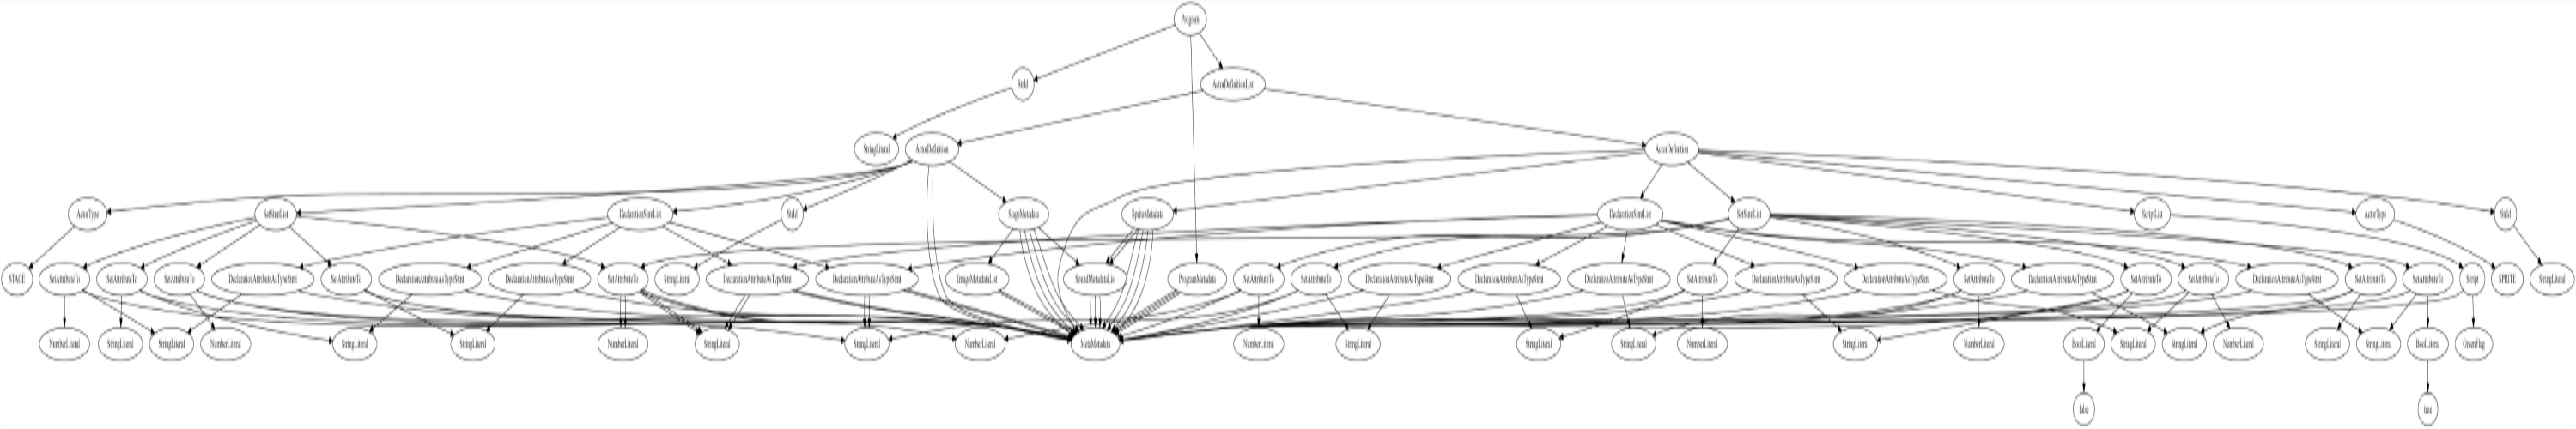
\includegraphics[scale=0.20]{images/AST_example(3).png}
\caption{Example AST structure of a simple \scratch\ project}
\label{fig:ast}
\end{figure}

For a simple \scratch{} project with only one [GreenFlag] block, the tree structure is already pretty big. This is caused by the amount of additional information nodes that are created by the \litterbox{} \AST{} but are not necessary or even part of the essential tokens that are needed for a \ngram{}. In Table~\ref{tab:excluded-metadata} is a quick overview of all \AST{-only} nodes that are for information purposes, whereas in Table~\ref{tab:excluded-blocks} are real \scratch\ blocks that exist in the \AST\ that were excluded because of their only usage in \textit{drop-down lists}. It is assumed that a programmer cannot choose falsely in a \textit{drop-down list} and because the list itself cannot be altered, all \textit{drop-down boxes} are seen as one token with their corresponding \scratch\ blocks. These nodes are all excluded for the tokenization in order to keep the n-gram model as small as possible and increase bug detection efficiency.   

\begin{table}[H]
    \caption[The excluded information-based \AST\ nodes]{\label{tab:excluded-metadata}The excluded information-based \AST\ nodes for tokenization of \scratch\ projects.}

    \begin{tabular}[t]{lll}
    	\toprule
    	Class & Type & Example \\
    	\midrule
    	\vspace{10pt}
    	    \texttt{ActorDefinition} & \texttt{AbstractNode} & Information storage of actor \\
    	    \vspace{10pt} 
    	    \texttt{ActorDefinitionList} & \texttt{AbstractNode} & List of \texttt{ActorDefinition} \\
    	    \vspace{10pt}
        \texttt{ActorType} & \texttt{ASTLeaf} & \texttt{STAGE, SPRITE} \\  
        \vspace{10pt}
        \texttt{DeclarationStmt} & \texttt{Stmt} & All types of attribute declarations\\
        \vspace{10pt}
        \texttt{Metadata} & \texttt{ASTNode} & \parbox[t]{7cm}{Additional information of the\\ \texttt{Program, Sprites, Stages, Resources, Blocks}} \\
        \vspace{10pt}
        \texttt{ProcedureDefinition} & \texttt{AbstractNode} & Definition of custom procedures \\
        \vspace{10pt}
        \texttt{ProcedureDefinitionList} & \texttt{AbstractNode} & List of \texttt{ProcedureDefinition} \\
        \vspace{10pt}
        \texttt{Program} & \texttt{AbstractNode} & Placeholder for a project\\
        \vspace{10pt}
        \texttt{Script} & \texttt{AbstractNode} & \texttt{Event} and \texttt{StmtList} of an actor \\  
        \vspace{10pt}
        \texttt{ScriptList} & \texttt{AbstractNode} & List of \texttt{Script} \\
        \vspace{10pt}
        \texttt{SetAttributeTo} & \texttt{AbstractNode} & Sets attributes at start of program \\
        \vspace{10pt} 
        \texttt{SetStmtList} & \texttt{AbstractNode} & List of attributes to set \\
        \vspace{10pt}
        \texttt{StmtList} & \texttt{AbstractNode} & List of \texttt{Stmt} \\
        \vspace{10pt}
        \texttt{StrId} & \texttt{LocalIdentifier} & Project ID \\            
    \bottomrule
    \end{tabular}
\end{table}

\begin{table}[H]
    \caption[The excluded \scratch\ blocks]{\label{tab:excluded-blocks}The excluded \scratch\ blocks for tokenization.}

    \begin{tabular}[t]{lll}
    	\toprule
    	Class & Type & Examples \\
    	\midrule
    	\vspace{10pt}
    		\texttt{Position} & \texttt{ASTNode} & \texttt{MousePos, RandomPos} \\
    		\vspace{10pt} 
    		\texttt{Backdrop} & \texttt{AbstractNode} & Backdrop1, Backdrop2,... \\
    		\vspace{10pt} 
    		\texttt{Costume} & \texttt{AbstractNode} & Costume1, Costume2,... \\
    		\vspace{10pt}
    		\texttt{DragMode} & \texttt{ASTLeaf} & \texttt{Not\_DRAGGABLE, DRAGGABLE} \\
    		\vspace{10pt}
   		\texttt{ElementChoice} & \texttt{ASTNode} & \texttt{Next, Prev, Random, WithExpr} \\
   		\vspace{10pt}
    		\texttt{ForwardBackwardChoice} & \texttt{ASTLeaf} & \texttt{FORWARD, BACKWARD} \\
    		\vspace{10pt}
    		\texttt{GraphicEffect} & \texttt{ASTLeaf} & \texttt{COLOR, GHOST, BRIGHTNESS,...} \\
    		\vspace{10pt}
    		\texttt{Key} & \texttt{AbstractNode} & \texttt{Spacebar, Arrow keys, Any,...} \\
    		\vspace{10pt} 
   	 	\texttt{LayerChoice} & \texttt{ASTLeaf} & \texttt{FRONT, BACK} \\ 
   	 	\vspace{10pt}
    		\texttt{Loudness} & \texttt{NumExpr, ASTLeaf} & \texttt{Integer} \\
    		\vspace{10pt}
   		\texttt{Message} & \texttt{AbstractNode} & Message1, Message2,... \\
   		\vspace{10pt}
    		\texttt{NumFunct} & \texttt{ASTNode, ASTLeaf} & \texttt{ABS, ACOS, ASIN, ATAN,...} \\
    		\vspace{10pt} 
   		\texttt{Rotation-Style} & \texttt{ASTLeaf} & \parbox[t]{7cm}{\texttt{Don't rotate, Left-right,\\ All around}} \\
   		\vspace{10pt}
    		\texttt{Size} & \texttt{NumExpr, ASTLeaf} & \texttt{Integer} \\
    		\vspace{10pt}
    		\texttt{SoundEffect} & \texttt{ASTLeaf} & \texttt{PAN, PITCH} \\
    		\vspace{10pt}
    		\texttt{TimeComp} & \texttt{ASTNode, ASTLeaf} & \texttt{DATE, DAY\_OF\_WEEK, HOUR,...} \\
    		\vspace{10pt}
    		\texttt{Timer} & \texttt{NumExpr, ASTLeaf} & \texttt{Integer} \\
    		\vspace{10pt} 
    		\texttt{Touchable} & \texttt{ASTNode} & \parbox[t]{7cm}{\texttt{Color, MousePointer, SpriteTouchable, Edge}} \\
    		\vspace{10pt}
    		\texttt{Variable} & \texttt{DataExpr} & My variable \\ 
    		\vspace{10pt}
        \texttt{Volume} & \texttt{NumExpr, ASTLeaf} & \texttt{Integer} \\     
    \bottomrule
    \end{tabular}
\end{table}

\section{N-gram Model Building in \scratch{}}\label{sec:model}
In the following sections the focus is on the building process of the \ngram{}, specifically in \scratch{}. Subsection~\ref{subsec:n-grams} goes in detail on how to calculate the probabilities of the found token sequences and add them to the growing model. The method of \textit{Smoothing} is then explained in Subsection~\ref{subsec:smoothing} as well as its importance in bug detection.

\subsection{Calculating and Adding N-grams}\label{subsec:n-grams}
First of all, the language model has to extract all possible token sequences in a \scratch{} project and calculate their probabilities like it is described in Subsection~\ref{subsec:n-grams}. This way a reliable probability distribution is created that will be the basis for later bug detection. 

For example, given the sequence [GreenFlag, Show, Hide] that is shown in Figure~\ref{fig:sequence}, all its consecutive subsequences are added to the model. In this case the subsequence [GreenFlag, Hide] that is shown in Figure~\ref{fig:subsequence} would be the only sequence that is ignored because [Hide] does not immediately follow [GreenFlag]. 

\begin{figure}%
    \centering
    \subfloat[A \scratch{} block sequence]{{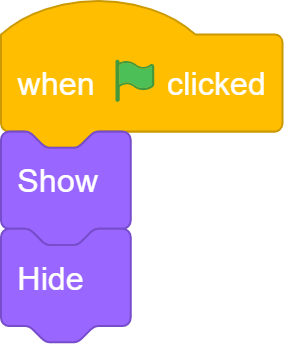
\includegraphics[width=5cm]{sequence.png} }\label{fig:sequence}}%
    \qquad
    \subfloat[Ignored subsequence]{{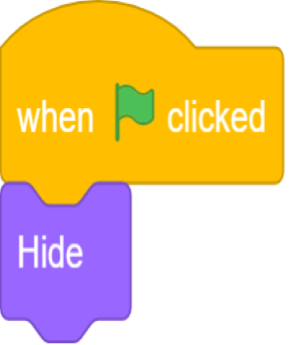
\includegraphics[width=5cm]{subsequence.png} }\label{fig:subsequence}}%
    \caption[\scratch{} block sequences]{\label{fig:sequences}\scratch{} block sequences}%
\end{figure}

If Figure~\ref{fig:sequence} would be the sequence we want to calculate the probability of, the estimation based on the \hyperref[def:markov_chain]{Markov chain} is executed by solving the Equation~\ref{eq:scratch-prob}. We are setting the \hyperref[def:gram size]{gram size} to 3 in this example. All internal probabilities are added by consulting the existing model and searching for the already calculated estimations. Therefore, the token sequence [GreenFlag, Show, Hide] can be calculated based on internal probabilities of its existing subsequences.

\begin{equation} \label{eq:scratch-prob}
\begin{aligned}
P([GreenFlag, Show, Hide]) ={} & P([GreenFlag])\cdot P([Show]|[GreenFlag]) \\
							  & \cdot P([Hide]|[GreenFlag, Show])
\end{aligned}
\end{equation}


\subsection{Smoothing of Probability Distribution}\label{subsec:smoothing}
If the analysed project is not part of the training dataset, it is important to smooth the probability distribution in order to avoid probabilities of zero. In this implementation, \textit{Add-One-Smoothing} was utilized which prevents non existent sequences to be shown by adding an additional count to each n-gram. All the counts that used to be zero will now have a count of 1, the counts of 1 will be 2, and so on. This algorithm is also called \textit{Laplace Smoothing}. This way there are no sequences with a probability of zero stored in the model that could affect the calculation of the sequence probabilities.

In the case of the unigram [GreenFlag], its maximum likelihood to appear in a \scratch{} project is estimated by counting the occurrences \textit{c} during the model training process and divide it through the total number of tokens \textit{N}. Therefore, the Equation~\ref{eq:likelihood} looks like this:

\begin{equation} \label{eq:likelihood}
P([GreenFlag]) ={} \frac{c}{N}
\end{equation}

\textit{Add-One-Smoothing} then, like the name suggests, only adds one to each count. Since there are a total of \textit{D} tokens in the model vocabulary and we added one more sighting to each one of them, we also have to adjust the denominator of the fraction accordingly. One more observation of each token means we have to increase the denominator by \textit{D}. If we apply the Math rules accordingly, the equation results in the following calculation in Equation~\ref{eq:laplace}:

\begin{equation} \label{eq:laplace}
P_{Laplace}([GreenFlag]) ={} \frac{c + 1}{N + D}
\end{equation}


\section{Bug Detection in \scratch{}}\label{sec:detection}
The specific algorithm to find bugs in \scratch{} is implemented the following way. At first, the probabilities of all sequences of the analysed project have to be calculated with help of the model like it is described in Subsection~\ref{subsec:n-grams}. After that, the sequences are ranked based on their probability and only the ones with the lowest probability get reported as potential bugs. In the next Subsection~\ref{subsec:configurations} all important parameters are set to ensure the optimal model analysis results. In Subsection~\ref{subsec:false_bugs} we found a method to minimize the amount of false positives in the reported bug set.

\subsection{Configurations}\label{subsec:configurations}
For the \scratch{} model implementation we added five parameters that have to be set accordingly in order to achieve the best evaluation results that are discussed later in Chapter~\ref{chap:evaluation}.

\paragraph{Gram Size.}
For probability calculations a \hyperref[def:markov_chain]{Markov chain} is used to get the conditional probability of a sequence using its n - 1 token predecessors as context information. In this work, n-gram models with a gram size between 2 to 4 are used in order to find the optimal n for bug detection in \scratch{} projects (Section \ref{sec:gram_size}). 
\paragraph{Sequence Length.}
In the same way we used a large dataset to obtain information about the best \hyperref[def:gram_size]{gram size n}, we also analysed which length of a token sequence could be the optimal size for a good model. Lengths from 2 to 6 were used to compare the different results of the n-gram bug detection. Finding the right length of a token sequence is evaluated in a more detailed way in Section \ref{sec:sequence_length}.
\paragraph{Reporting Size.}
In this implementation the reporting size for the big dataset model from Subsection~\ref{subsec:trainingset} is fixed at 25 reports per analysis, whereas we did not limit the reporting size for the small dataset that  is further introduced in Subsection~\ref{subsec:bugset}. One reason for this decision was that if the reporting size is chosen too big, the risk of false positives is also increased. Furthermore, the amount of reported bugs is very small in the case of the second set because the projects as well as the model itself are not very big. If we would have restricted the amount of reported bugs even more, there would not be enough output created to analyse.  
\paragraph{Minimum Token Occurrence.}
In this bachelor's thesis \ngram{} which is only for \scratch{} analysis purposes the minimum token occurrence is chosen as one. Because of the size difference between usual Java projects compared to normal \scratch{} projects, it would not make sense to filter out any tokens. \scratch{} programmers do not have as much freedom in their implementation because of the restriction through a block-based language and usually choose a different purpose for their programs than text-based programming languages would, which leads to much smaller projects with fewer usages of specific tokens. So, the minimum token occurrence parameter would only make it harder to find low probability sequences in projects which is why we decided not to raise this threshold for the analysis.
\paragraph{Probability Threshold.}
If a sequence in the report has a probability that is higher than the given threshold, it probably is a normal token sequence that just happens to have a lower probability than the rest of the project's blocks. In this implementation, the threshold is fixed at 0.05 for the big dataset of Subsection~\ref{subsec:trainingset} and at 0.6\% or 1.6\% for the pupils' projects of Subsection~\ref{subsec:bugset}. The reason is again the size difference that would minimize the analysis output even more, if this restriction would be too low for the small project set.

\subsection{Pruning False Bugs}\label{subsec:false_bugs}
Token sequences with low probability are at the bottom of a n-gram reporting list for potential bugs. But there is always the chance that the found sequence is not actually wrong but just a very unusual or special use case in which its probability would also rank rather low. To find and filter out this kind of false bugs and reduce the candidate bug set, token sequences can only be reported when they are at the bottom of at least two ranked lists of \ngram{s} with the same \textit{gram size} but different \textit{sequence lengths}. This way, sequences are sorted out that just appear on one of these lists and the chance to report false positives gets drastically reduced. 


\section{Implementation}\label{sec:implementation}
This section explains the tool chain of our approach for \ngram{} in \scratch\ and clarifies implementation
decisions. Table~\ref{tab:ngram-params} gives an overview over the model building process in \scratch, the bug detection system, the parameters which can be adjusted, and the input and output of each step.

\begin{table}[H]
    \caption[The tool chain for N-gram bug detection in \scratch]{\label{tab:ngram-params}The tool chain for N-gram bug detection in \scratch.}

    \begin{tabular}[t]{lllll}
        \toprule
        \parbox{2cm}{Steps} & Input & Tool & \parbox{2cm}{Output\\format} & Parameters \\
        \midrule
        \vspace{10pt}
        
        \parbox[t]{2cm}{Model\\ Building} &\parbox[t]{2.5cm}{\scratch\ dataset,\\ \texttt{model.csv}} & \parbox[t]{3cm}{\ngramtrainer{}, \tokenizer{}} & \parbox[t]{2cm}{\texttt{.csv}} & \parbox[t]{3.8cm}{\hyperref[def:gram_size]{gram size}}\\
        
        \vspace{10pt}
        
        \parbox[t]{2cm}{Bug\\ Detection} & \parbox[t]{2.5cm}{\scratch\ \\ bug set,\\ \texttt{model.csv},\\ \texttt{report.csv}} & \parbox[t]{3cm}{\ngrambugfinder{}, \tokenizer{}} & \parbox[t]{2cm}{\texttt{.csv}} & \parbox[t]{3.8cm}{\hyperref[def:report_size]{report size},\\ \hyperref[def:gram_size]{gram size},\\ 	\hyperref[def:sequence_length]{sequence length},\\ \hyperref[def:probability_threshold]{probability \\ threshold},\\ with/without smoothing}\\ 

        \bottomrule
    \end{tabular}
\end{table}

\subsection{\tokenizer{}}\label{subsec:tokenizer}
The basis of the n-gram building process is to tokenize each project and structure in the same way. The \ngramtrainer\ as well as \ngrambugfinder\ both use \litterbox\ to create an \AST\ for a given program. The \AST\ then maps every command block to a corresponding \AST\ node. In this process every \textit{hat block} is implementing the interface \texttt{Event} and all remaining \textit{command blocks} are associated with the \texttt{Stmt} interface. For instance, the [Turn Right] block is represented by an object of the \texttt{TurnRight} class which implements the \texttt{Stmt} interface. A visitor then visits the \AST\ and partitions the project into its \hyperref[def:token]{tokens}.

\subsection{\ngramtrainer{}}\label{subsec:ngramtrainer}
\ngramtrainer, a feature added to \litterbox, creates a \ngram\ of a set of \scratch\ projects. The model stores a probability distribution of all token sequences that were found in the training set. It is then utilized as a foundation for bug detection in \scratch.

The model creation process consists of three steps: First, all possible sequences of tokens that can be created of the analysed training set are calculated, counted, and stored in a \texttt{Map} structure. Second, we go through the \texttt{Map} of sequences and estimate the probability of each sequence, like it is shown in Equation~\ref{eq:likelihood}, by counting the amount a sequence appeared during the n-gram calculation and dividing it by the total number of sequences. After the calculation the finished model is printed as a \texttt{.csv} file and is ready for its usage in further analysis and bug detection procedures.

\subsection{\ngrambugfinder{}}\label{subsec:ngrambugfinder}
\ngrambugfinder, another extension that was added to \litterbox, continues the analysis process of the \ngramtrainer\ by using its calculated model. First, to find bugs in a project, the project itself is partitioned into sequences of a specific length that are stored in a \texttt{Map}. Then the probability of each sequence is estimated with help of the given probability distribution of the n-gram model. The probabilities are then ranked and the sequences with the lowest score are reported as potential bugs. The final \texttt{.csv} file then shows the reported sequences with their location information and calculated probabilities.
% !TeX spellcheck = en_GB
% !TeX encoding = UTF-8
% !TeX root = ../thesis.tex

\newcommand{\numlarge}{75,277}
\newcommand{\monthstart}{December 2019}
\newcommand{\monthend}{January 2020}
\newcommand{\parsingexcp}{114}
\newcommand{\successfullyanalysed}{74,914}
\newcommand{\calculatedngrams}{138,298}
\newcommand{\creationtime}{17 days}

\chapter{Evaluation}\label{chap:evaluation}

The main research points for this bachelor's thesis are answers to the following questions:
\begin{itemize}
\item[\textbf{RQ1}] How effective are \ngram{s} for bug detection in comparison to \litterbox{}?
\item[\textbf{RQ2}] What kinds of violations were detected by the \ngram{}?
\item[\textbf{RQ3}] Does the \ngram\ work in the case of open task solutions?
\item[\textbf{RQ4}] Efficiency of general \ngram\ vs project-specific model?
\end{itemize}

In the following analysis, parameters for the \ngram\ configuration were determined, like it is described in Subsection~\ref{subsec:configurations}. The \hyperref[def:gram_size]{\textit{gram size}} of 3 is adopted from the \bugram{}~\cite{bugram} paper. For the \hyperref[def:sequence_length]{\textit{sequence length}} we got the best results with the lengths 2 and 3. Furthermore, the \hyperref[def:probability_threshold]{\textit{probability threshold}} was manually estimated for each \ngram{}. The value that distinguished the most true bugs from false positives was chosen.


\section{Data Sets and Models}\label{sec:dataset}
RQ1, RQ2 and RQ3 are all answered by using project-specific models (Subsection~\ref{subsec:bugset}) and analysing representative projects of different pupil tasks. In RQ4 the general model (Subsection~\ref{subsec:trainingset}) which is based on a bigger data set is compared to the reports of the project-specific models.

\subsection{Big Data Set}\label{subsec:trainingset}
In order to have a sufficient number of sequences to calculate a probability distribution from and as comparison to the smaller project-specific models, we decided to build an \ngram{} on a large data set with its statistics shown in Table~\ref{tab:general-model}. The dataset consists of \numlarge\ \scratch\ projects. From \monthstart\ to \monthend\ we downloaded the most recent projects with the \scratch\ REST API\footnote{\url{https://github.com/LLK/scratch-rest-api/wiki}, last accessed May 8, 2020}. We did exclude remixes from the data set. \litterbox\ could not parse \parsingexcp\ projects, thus the \ngram\ was created of \successfullyanalysed\ projects without any exceptions and consists of \calculatedngrams\ calculated n-grams. The creation of the model took \creationtime\ and was conducted on machines equipped with Intel Xeon E5-2650 v2 @ 2.60 GHz CPUs with 256 GiB of RAM.

\begin{table}[hbtp]
    \centering
    \caption[General model statistics]{\label{tab:general-model}General model statistics.}
    \begin{tabular}{lrrr}
        \toprule
        File & Size & \#Projects & \#Ngrams\\
        \midrule
        \texttt{model.csv} & 7,865 KB & 74,914 & 138,298 \\
        \bottomrule
    \end{tabular}
\end{table}

\subsection{Pupil's Projects}\label{subsec:bugset}
The creation of the project-specific models as well as bug detection with the pupil's projects was done in a few seconds for every set of solutions and did not throw any exceptions. All experiments with the small data sets were conducted on a Swift SF314-57 with an Intel i5 core and 8 GB RAM.

\paragraph{Project-specific Models.}
The project-specific models with further statistics shown in Table~\ref{tab:specific-model} are build on a set of correct as well as defective solutions of five small coding tasks for students. Based on the task the pupils had to implement, we call these sets \textit{Monkey}, \textit{Elephant}, \textit{Cat}, \textit{Horse} and \textit{Fruit Catching} task. We used solutions of pupils which originate in primary programming education~\cite{katharina} for the \textit{Monkey}, \textit{Elephant}, \textit{Cat} and {Horse} tasks. For the \textit{Fruit Catching} task we used the same data set as Stahlbauer et al. in their work about testing \scratch\ programs automatically~\cite{whisker}. In addition, a set of open task solutions that pupil's could experiment with was used for Section~\ref{sec:open}. 

\begin{table}[hbtp]
    \centering
    \caption[Project-specific model statistics]{\label{tab:specific-model}Project-specific model statistics.}
    \begin{tabular}{lrrrr}
        \toprule
        Task & File & Size & \#Projects & \#Ngrams \\
        \midrule
        Fruit Catching & \texttt{fruit\_model.csv} & 226 KB & 42 & 3,257  \\
        Monkey & \texttt{monkey\_model.csv} & 33 KB & 120 & 477 \\
        Elephant & \texttt{elephant\_mode.csv} & 39 KB & 130 & 559 \\
        Cat & \texttt{cat\_model.csv} & 49 KB & 129 & 715 \\
        Horse & \texttt{horse\_model.csv} & 30 KB & 73 & 440 \\
        Open & \texttt{open\_model.csv} & 101 KB & 295 & 1,897 \\
        \bottomrule
    \end{tabular}
\end{table}

\paragraph{Bug Detection.}
For bug detection we chose one representative project of each task which are listed in Table~\ref{tab:buggy-projects} and analysed them with \litterbox\ as well as the created n-gram models for the research questions. 

\begin{table}[hbtp]
    \centering
    \caption[Representative projects of each task for bug detection]{\label{tab:buggy-projects}Representative projects for each task used for bug detection.}
    \begin{tabular}{lrrrr}
        \toprule
        Task & Project & Size & \#Sprites & \#Blocks\\
        \midrule
        Fruit Catching & \texttt{K7\_S02.sb3} & 176 KB & 3.0 & 81.0\\
        Monkey & \texttt{ID\_065\_Aufgabe-Affenjagd.sb3} & 181 KB & 3.0 & 18.0 \\
        Elephant & \texttt{ID\_118\_Aufgabe-Elefant.sb3} & 456 KB & 4.0 & 23.0 \\
        Cat & \texttt{ID\_005\_Aufgabe-Katze.sb3} & 86 KB & 2.0 & 14.0 \\
        Horse & \texttt{ID\_080\_Aufgabe-Pferd.sb3} & 6 KB & 1.0 & 14.0 \\
        Open & \texttt{m043.sb3} & 304 KB & 3.0 & 26.0 \\ 
        Open & \texttt{m052-Zauberei.sb3} & 869 KB & 7.0 & 18.0 \\
        Open & \texttt{m067-Apfelsuche.sb3} & 330 KB & 3.0 & 31.0 \\
        Open & \texttt{m074-Sternenjaeger.sb3} & 58 KB & 12.0 &  65.0 \\
        Open & \texttt{m091 2.sb3} & 53 KB & 7.0 & 70.0 \\
        Open & \texttt{w002-Weltraumangriff.sb3} & 703 KB & 7.0 & 57.0 \\
        \bottomrule
    \end{tabular}
\end{table}

\paragraph{Project-specific Model Reports.}
The created boxplot in Figure~\ref{fig:boxplot1} visualises a distribution of the reported sequences for all pupil projects. We can see that each task has a different number of sequences that were detected as potential bugs with the \textit{Fruit Catching} task being the one with the most reported sequences. The huge difference between the \textit{Fruit Catching} task and the rest of the tasks is probably related to its big block counts in the projects which ultimately leads to a higher number of reported sequences.

\begin{figure}[hbtp]
    \centering
    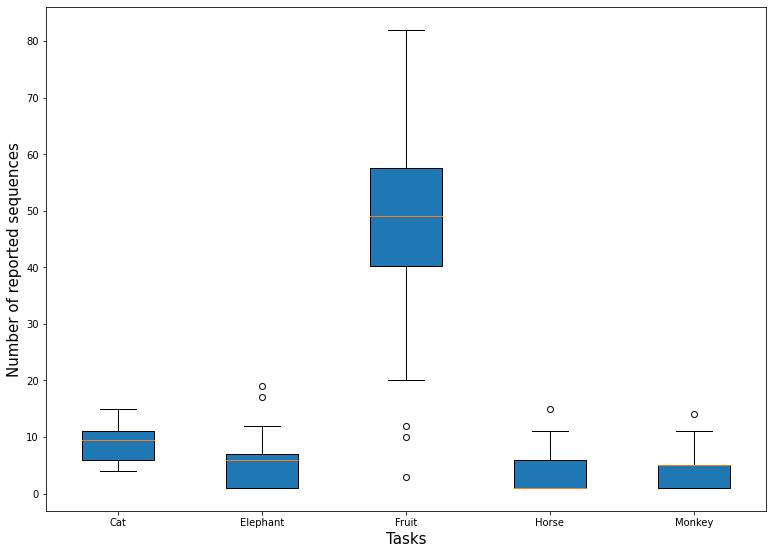
\includegraphics[scale=0.4]{boxplot_sequences.png}
    \caption[Boxplot for distribution of reported sequences]{\label{fig:boxplot1}Boxplot for distribution of reported sequences.}
\end{figure}

As a comparison to Figure~\ref{fig:boxplot1}, Figure~\ref{fig:boxplot2} shows a distribution of all reported sequences that have an occurrence probability below the estimated \hyperref[def:probability_threshold]{\textit{probability thresholds}} and therefore are more likely to be true bugs or unusual use cases than false positives.

\begin{figure}[hbtp]
    \centering
    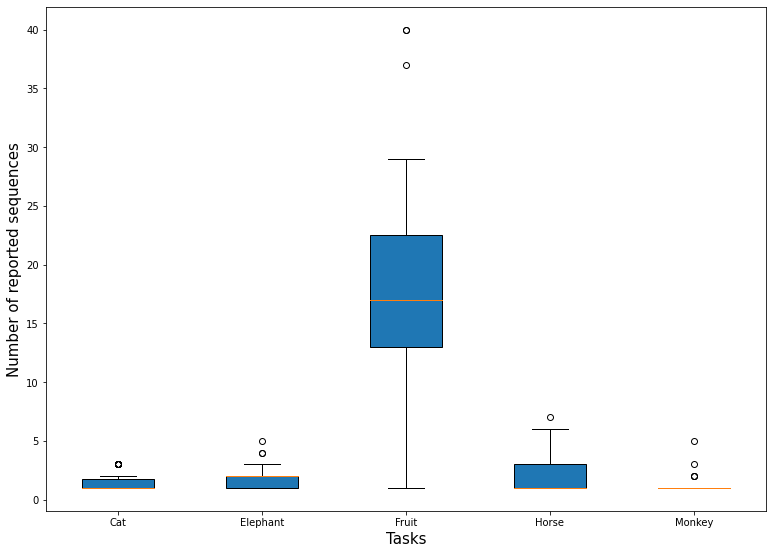
\includegraphics[scale=0.4]{boxplot_threshold.png}
    \caption[Boxplot for distribution of reported sequences with probability thresholds]{\label{fig:boxplot2}Boxplot for distribution of reported sequences with probability thresholds.}
\end{figure}

\begin{figure}[hbtp]
    \centering
    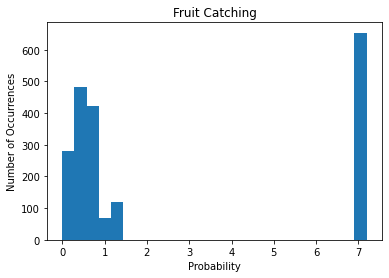
\includegraphics[scale=0.5]{fruit_his.png}
    \caption[Histogram for probability distribution of \textit{Fruit Catching} task]{\label{fig:fruit_his}Histogram of \textit{Fruit Catching} task with a \hyperref[def:probability_threshold]{\textit{probability threshold}} of 0.6\%.}
\end{figure}

\begin{figure}[hbtp]%
    \centering
    \subfloat{{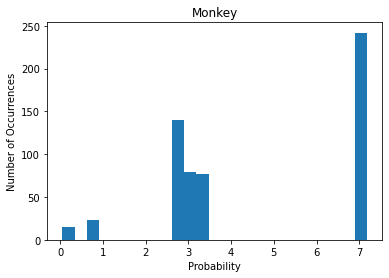
\includegraphics[width=7cm]{monkey_his.png} }}%
    \qquad
    \subfloat{{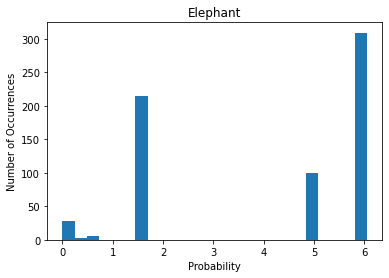
\includegraphics[width=7cm]{elephant_his.png} }}%
    \caption[Histograms of \textit{Monkey} and \textit{Elephant} tasks]{\label{fig:his1}Histograms of \textit{Monkey} and \textit{Elephant} tasks with a  \hyperref[def:probability_threshold]{\textit{probability threshold}} of 1.6\%.}%
\end{figure}

\begin{figure}[hbtp]%
    \centering
    \subfloat{{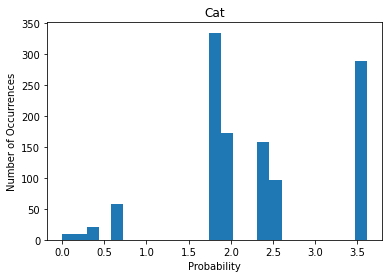
\includegraphics[width=7cm]{cat_his.png} }}%
    \qquad
    \subfloat{{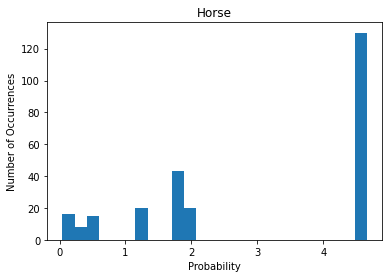
\includegraphics[width=7cm]{horse_his.png} }}%
    \caption[Histograms of \textit{Cat} and \textit{Horse} tasks]{\label{fig:his2}Histograms of \textit{Cat} and \textit{Horse} tasks with a  \hyperref[def:probability_threshold]{\textit{probability threshold}} of 1.6\%.}%
\end{figure}

The histograms of Figures~\ref{fig:fruit_his}, ~\ref{fig:his1} and ~\ref{fig:his2} show the probability distributions of the reported sequences for each task. The estimated \hyperref[def:probability_threshold]{\textit{probability thresholds}} can be seen in the figures as separations of low probability sequences to usual occurrences. A manual examination confirmed that below the chosen  \hyperref[def:probability_threshold]{\textit{probability thresholds}} the probability of false positives is very small.


\section{RQ1: Comparison to Litterbox}\label{sec:litterbox}
After setting the \hyperref[def:gram_size]{\textit{gram size}} to 3 and \hyperref[def:sequence_length]{\textit{sequence lengths}} to 2 for the first analysis and 3 for the second bug detection analysis, project-specific models for each pupil task from Table~\ref{tab:specific-model} are used for a comparison between \litterbox~\cite{scratch_bugpatterns} and the \ngram{} approach of \bugram~\cite{bugram}. The same projects from Table~\ref{tab:buggy-projects} are analysed by \litterbox{} and the \ngram{} to test how many sequences are reported after knowing the failed tests of each project through \whisker~\cite{whisker}. The \hyperref[def:reporting_size]{\textit{reporting size}} is unlimited in this case. Table~\ref{tab:litterbox} shows the number of reported smells or sequences of each method. 

\begin{table}[hbtp]
    \centering
    \caption[The number of reported bugs found by \litterbox{} and n-gram model]{\label{tab:litterbox}The number of reported bugs found by \litterbox{} and n-gram model.}
    \begin{tabular}{lrrr}
        \toprule
        Task & \#FailedTests & \#LitterboxSmells & \#NgramSequences \\
        \midrule
        Fruit Catching & - & 113 & 42 \\
        Monkey & 0 & 2 & 8 \\
        Elephant & 0 & 1 & 5 \\
        Cat & 0 & 0 & 6 \\
        Horse & 1 & 0 & 8 \\
        \bottomrule
    \end{tabular}
\end{table}

The analysis shows that even though in some cases \litterbox\ did not find smells and \whisker\ tests all passed, the \ngram\ reported sequences that pointed out potential bugs or unusual use cases. This shows that the \ngram\ has a different range of violations it can detect in \scratch\ projects.


\section{RQ2: Violation Classification}\label{sec:violations}
The analysis procedure is continued by analysing specifically the bugs that are reported by the \ngram{}. For each task one project is manually analysed to estimate the rate of false positives. The \hyperref[def:probability_threshold]{probability threshold} varies from the size of the model. Table~\ref{tab:buggy-projects} shows the projects that were chosen for assessment as well as their further information. After all by the \ngram{} detected potential bugs were collected in the candidate bug set, the defective code is manually classified into the following categories: \textit{True Bugs}, \textit{Unusual Use Cases} or \textit{False Positives}. Table~\ref{tab:violations} displays the numbers for each category.

\begin{table}[hbtp]
    \centering
    \caption[The categorization of all reported bugs]{\label{tab:violations}The categorization of all reported bugs.}
    \begin{tabular}{lrrrrr}
        \toprule
        Task & \parbox[t]{2.2cm}{Probability\\Threshold} & \#Reported & \#True & \#UnusualUse & \#FalsePositive \\
        \midrule
        Fruit Catching & 0.6\% & 23 & 15 & 3 & 5 \\
        Monkey & 1.6\% & 3 & 2 & 1 & 0 \\
        Elephant & 1.6\% & 1 & 0 & 1 & 0 \\
        Cat & 1.6\% & 1 & 0 & 1 & 0 \\
        Horse & 1.6\% & 4 & 3 & 0 & 1 \\
        \bottomrule
    \end{tabular}
\end{table}

If a sequence is an unusual use case, it will not be detected by \litterbox\ because it is not a code smell. Most of the time an unusual use is a consequence of an extension of the original task and therefore not part of the usual used sequences that are needed for a project to pass the test. 

\begin{table}[hbtp]
    \centering
    \caption[An excerpt of the report for the \textit{Fruit Catching} task]{\label{tab:report}An excerpt of the report for the \textit{Fruit Catching} task.}
\begin{tabular}{lrrr}
        \toprule
        Actor & Position & Sequence & Probability\\
        \midrule
        Bowl & Script@1608d14c & RepeatTimesStmt, NumberLiteral & 0.06948304613674264 \\
	   Apple & Script@1ff8da & Never, UntilStmt & 0.44469149527515284 \\
	   Apple & Script@3a4e11a & IfElseStmt, UnspecifiedBoolExpr & 0.023346303501945526 \\
	   Apple & Script@e3e2beb8 & ChangeYBy, NumberLiteral & 0.39355197331851033 \\
        \bottomrule
    \end{tabular}
\end{table}

\begin{figure}[hbtp]%
    \centering
    \subfloat[Example \scratch\ code.]{{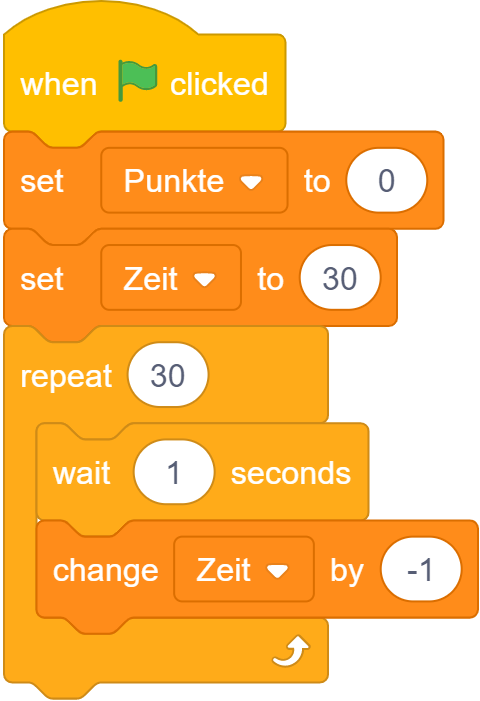
\includegraphics[width=5cm]{unusualUse.png} }}%
    \qquad
    \subfloat[RepeatTimesStmt, NumberLiteral]{{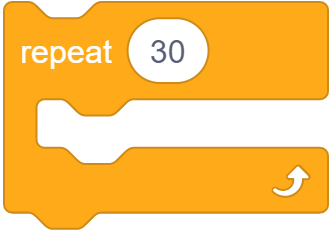
\includegraphics[width=5cm]{reportedUnusualUse.png} }}%
    \caption[Example \textit{script} for detected unusual use case in \scratch\ code]{\label{fig:unusualUse}Example \textit{script} for detected unusual use case in \scratch\ code.}%
\end{figure}

Figure~\ref{fig:unusualUse} from the project \texttt{K7\_S02.sb3} shows an example for an unusal use case with the sequence [RepeatTimesStmt, NumberLiteral] that was reported with a probability of 0.07\%, according to the report excerpt in Table~\ref{tab:report}. This means that in the solutions of the \textit{Fruit Catching} task, the usage of a [RepeatTimesStmt] block was very limited and therefore it is despite its low probability not a bug.  

\begin{figure}[H]
    \centering
    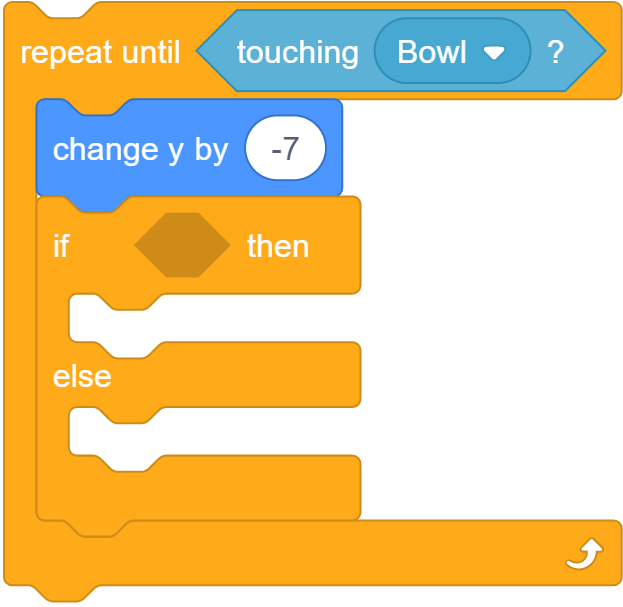
\includegraphics[scale=0.4]{trueBug.png}
    \caption[Example for detected bug and false positive in \textit{Fruit Catching} project]{\label{fig:trueBug}Example for detected bug and false positive in \textit{Fruit Catching} project.}
\end{figure}

Another example would be the \textit{script} in Figure~\ref{fig:trueBug} where everyone can see at first glance that there is a bug that is caused by missing \textit{blocks}. The reported sequences, that are also shown in Table~\ref{tab:report}, are [Never, UntilStmt] with 0.44\%, [IfElseStmt, UnspecifiedBoolExpr] with a probability of 0.02\% and [ChangeYBy, NumberLiteral] with 0.39\% although the last sequence is classified as a false positive. 

When we compare the code smells that \litterbox\ is able to find with the bugs that can be detected by the \ngram{}, then we see that the \ngram\ is not able to detect long scripts or unused variables in the \scratch\ code. But the \ngram\ is capable of finding dead code, empty scripts as well as empty bodies in if-else statements. 
 

\section{RQ3: Open Solutions}\label{sec:open}
For a wider perspective on the usage of the \ngram\ approach to bug detection we selected a set of pupil's solutions where the children could try out all the things they had newly learned. This means that there is no unique solution for these tasks, just open interpretations of simple projects. Therefore there is no method to determine if a reported sequence is an unusual use case. The project-specific model, we created out of the solutions, reported the following bugs displayed in Table~\ref{tab:open} for a set of example projects of the data set. In this analysis the \hyperref[def:probability_threshold]{\textit{probability threshold}} is set to 0.5\% for the model. 

\begin{table}[hbtp]
    \centering
    \caption[Open projects report]{\label{tab:open}Reported bugs of open projects.}
    \begin{tabular}{lrrr}
        \toprule
        Task & \#Reported & \#TrueBug & \#FalsePositive \\
        \midrule
        \texttt{m043.sb3} & 4 & 3 & 1 \\   
        \texttt{m052-Zauberei.sb3} & 2 & 1 & 1 \\ 
        \texttt{m067-Apfelsuche.sb3} & 1 & 0 & 1 \\
        \texttt{m074-Sternenjaeger.sb3} & 1 & 0 & 1 \\
        \texttt{m091 2.sb3} & 4 & 0 & 4 \\
        \texttt{w002-Weltraumangriff.sb3} & 2 & 2 & 0 \\            
        \bottomrule
    \end{tabular}
\end{table}

The frequent occurrence of false positives could be a consequence of the missing unusual use case categorisation. A lot of sequences just were not used as often by the novice programmers and when they appear one time their probability is consequently pretty low. 

\begin{table}[hbtp]
    \centering
    \caption[An excerpt of the report for the \textit{Zauberei} task]{\label{tab:report2}An excerpt of the report for the \textit{Zauberei} task.}
\begin{tabular}{lrrr}
        \toprule
        Actor & Position & Sequence & Probability\\
        \midrule
    	   Rokkduck & Script@497b81c5 & PlaySoundUntilDone, Never & 0.16643473084111865 \\
        Rokkduck & Script@497b81c5 & RepeatTimesStmt, NumberLiteral & 0.3615592433603648 \\
        \bottomrule
    \end{tabular}
\end{table}

\begin{figure}[hbtp]
    \centering
    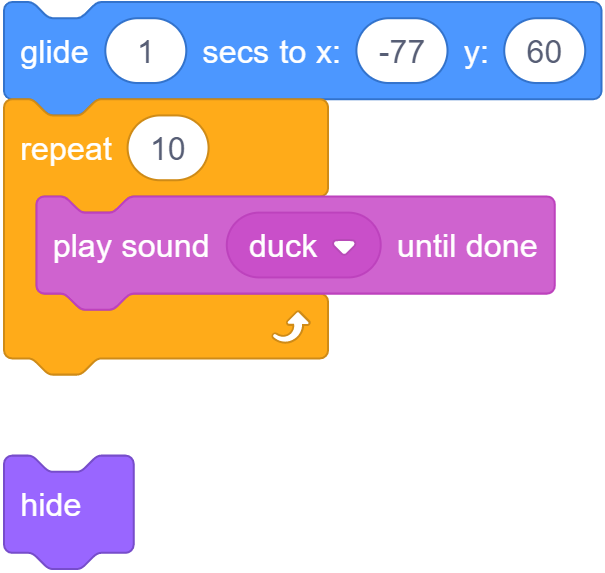
\includegraphics[scale=0.4]{openBugs.png}
    \caption[Example for detected bug and false positive in open project]{\label{fig:openBugs}Example for detected bug and false positive in open project.}
\end{figure}

The \scratch\ \textit{script} in Figure~\ref{fig:openBugs} is a part of the \texttt{m052-Zauberei.sb3} code and contains an example for a bug as well as false positive that are shown in the report excerpt in Table~\ref{tab:report2}. The sequence [PlaySoundUntilDone, Never] with a probability of 0.17\% is a bug because it hints at the [Hide] block that can never be executed because of a missing \textit{hat} block. Furthermore, the sequence [RepeatTimesStmt, NumberLiteral] with 0.36\% is falsely reported because it is not a programming mistake. If there was a reference solution of the \textit{Zauberei} task, then it could also be an unusual use case depending on the number of occurrences of the [RepeatTimesStmt] block in the solutions.


\section{RQ4: General vs Project-specific Model}\label{sec:project-specific}
The bigger model may have a wider range of potential n-grams but this does not correlate with better results. Like it is shown in Table~\ref{tab:versus} with the \textit{Cat} task as an example, the reported probabilities of the general model are not usable in a way to identify potential bugs, code smells or unusual use cases in the \scratch\ code in comparison to project-specific models. 

\begin{table}[hbtp]
    \centering
    \caption[General vs project-specific model]{\label{tab:versus}General vs project-specific model.}
    \begin{tabular}{lrr}
        \toprule
        Sequence & General & Project-specific \\
        \midrule
        GreenFlag, RepeatForeverStmt & -163.7176695714846 & 0.0052368762629570725 \\
        Touching, SayForSecs & -93.4693467460925 & 0.0025830339970531286 \\
        PointTowards, MoveSteps & -56.557244922395064 & 3.548409418312439E-4 \\
        NumberLiteral, IfThenStmt & 72.48561394813275 & 0.0033964044507544403 \\
        NumberLiteral & 72.48561394813275 & 2.3721578534715566 \\
        StringLiteral, NumberLiteral & -46.75499727794927 & 0.0027517806291449814 \\
        \bottomrule
    \end{tabular}
\end{table}

One reason are negative possibilities that appeared in the reports. The origin of the negative calculations are still unclear and have to be analysed in a more thorough way in the near future. A programming mistake or miscalculations could be the reason but even in the case of a correct probability estimation, project-specific n-gram models are more reliable in their usage.  


\section{Threats to Validity}\label{sec:threats-to-validity}
There is no guarantee that this bachelor's thesis is free of faults or miscalculations. Here are a few points that should be addressed about the here described and executed research as well as evaluation of the \ngram{} on \scratch{} code.

\paragraph{Implementation of N-gram Model.}
To compare the results of \litterbox{} with the n-gram model approach, we implemented the n-gram language model as close as possible to the information given from the \bugram{}~\cite{bugram} paper and based on the \AST{} that is created by \litterbox{} out of \scratch{} projects in JSON format. For our implementation, we have tried our best to tune the configuration parameters to obtain the best results. Our comparison is fair because both \litterbox{} as well as \ngram{} are evaluated on the same projects.

\paragraph{Bugs are manually verified.}
Following the \bugram{}~\cite{bugram} paper, reported bugs were assessed manually in order to approve and classify all low probability \hyperref[def:token]{\textit{token}} sequences and distinguish between, i.e., true bugs, unusual use cases and false positives. Since we are not the original programmers of the analysed projects that are featured in this bachelor's thesis, the examination of the code is not objective. But because of common practice, it is an acceptable approach for the assessment of the given code.
% !TeX spellcheck = en_GB
% !TeX encoding = UTF-8
% !TeX root = ../thesis.tex
\chapter{Discussion}\label{ch:discussion}
The next Section~\ref{sec:threats-to-validity} touches on the reason why there are threats to the credibility and accuracy of the bachelor's thesis. There are also further works of literature that talk about similar topics that were discussed in this thesis which are summarized in small introductions in Section~\ref{sec:related-work}.

\section{Threats to Validity}\label{sec:threats-to-validity}
There is no guarantee that this bachelor's thesis is free of faults or miscalculations. Here are a few points that should be addressed about the here described and executed research as well as evaluation of the \ngram{} on \scratch{} code.

\paragraph{Implementation of N-gram Model.}
To compare the results of \litterbox{} with the n-gram model approach, we implemented the n-gram language model as close as possible to the information given from the \bugram{}~\cite{bugram} paper and based on the \AST{} that is created by \litterbox{} out of \scratch{} projects in JSON format. For our implementation, we have tried our best to tune the configuration parameters to obtain the best results. Our comparison is fair because both \litterbox{} as well as \ngram{} are evaluated on the same projects.

\paragraph{Bugs are manually verified.}
Following the \bugram{}~\cite{bugram} paper, reported bugs were assessed manually in order to approve and classify all low probability token sequences and distinguish between, i.e., true bugs, refactoring opportunities and false positives. Since we are not the original programmers of the analysed projects that are featured in this bachelor's thesis, the examination of the code is not objective. But because of common practice, it is an acceptable approach for the assessment of the given code.

\section{Related Work}\label{sec:related-work}
The analysis of code in order to obtain information and improve its efficiency and readability is a common method of reducing bug patterns and code smells. These are a few examples of specific ways how researchers try to increase their knowledge about written code and how to get better results in the long term independent of the assessed programming languages.

\paragraph{Analysing \scratch{} Programs}
The tools \drscratch{}~\cite{drscratch} as well as \hairball{}~\cite{hairball} analyse \scratch{} programs to find bugs and code smells. These are then reported to the user in order to improve the computational thinking and coding skills of novice programmers. Bad programming habits were assessed in a preliminary study by Moreno et al.~\cite{badhabits} and code smells that are very common in Scratch were analysed by Vargas-Alba et al.~\cite{badsmells}. Stahlbauer et al.~\cite{whisker} introduced \whisker{} which is a formal testing framework for Scratch. \litterbox, a tool created by Frädrich et al.~\cite{scratch_bugpatterns} that creates an \AST\ of \scratch{} programs, is used for finding code smells as well as bug patterns.

\paragraph{Object Usage Anomalies}
Interactions with objects are required to follow a specific procedure, for example by a sequence of method calls. But these standards are rarely documented and can lead to problematic behaviour in the code. Wasylkowski et al.~\cite{object_usage} infers legal sequences of method calls to code examples. The results can then be used to find anomalies in the analysed implementation. As a automatic defect detection algorithm, it is the first of its kind that uses method call sequences to learn and detect anomalies.

\paragraph{N-gram Language Models}
Hindle et al.~\cite{naturalness} first introduced the \ngram{} to show that software source code is highly repetitive and the \ngram{} can be used in code suggestion and completion. This work is the basis for using language models to model source code and demonstrated how they could be used in software tools. A very accurate algorithm by using a Hidden Markov Model for code completion was proposed by Han et al.~\cite{codecompletion}. SLAMC by Nguyen et al.~\cite{SLAMC}, which incorporated semantic information into a n-gram model, presented a method to code suggestion. It demonstrated how tokens can be seen more semantically instead of just syntactically. Raychev et al.~\cite{SLANG} investigated the effectiveness of various language models for code completion, i.e., n-gram and recurrent neural networks. By combining program analysis and the n-gram model, they proposed SLANG, which had the goal to predict the sequence of method calls in a software system. 

\paragraph{\bugram{}}
The effective usage of n-gram language models in the field of bug detection is also demonstrated by Wang et al.~\cite{bugram} with their tool \bugram{} that finds defective code with \ngram{s} in \java{} programs. Although there are other studies that covered the usage of n-grams for detecting clone bugs~\cite{clonebugs}, localizing faults~\cite{faults} and code search~\cite{codesearch}, these did not leverage n-gram models. In contrast to n-grams that are only token sequences, n-gram models are Markov models built on n-grams.
% !TeX spellcheck = en_GB
% !TeX encoding = UTF-8
% !TeX root = ../thesis.tex
\chapter{Conclusion}\label{chap:conclusion}
%TODO Unfinished chapter!

Writing code can be a frustrating experience when the tools given are not enough to ensure that the created program fulfils all the important requirements to run smoothly and without mistakes. Even more so when the programmers are pupils who are in the beginner state of understanding what coding really means. \scratch\ already is a good starting platform to learn the basics but the editor misses essential debugging tools.

To improve the accuracy of \scratch\ projects and lessen the frustration that comes with bug detection, this bachelor's thesis proposed a method of bug detection that is based on \ngram{s}. The \tokenizer\ uses the \AST\ of \litterbox\ as a foundation for tokenizing each \scratch\ project. By calculating a probability distribution of all n-grams in a given dataset, the \ngramtrainer\ is then able to estimate the probability of the occurrence of a specific token sequence that is used in \scratch\ projects. Assuming that a low probability hints at a programming mistake or an unusual use case, the \ngrambugfinder\ can analyse projects based on the \ngram\ that was calculated by the \ngramtrainer\ and report these sequences as potential bugs.

We created a \ngram\ out of a big data set that consists of 75,277 as well as small sets of pupil's solutions for common tasks. At first we used project-specific \ngram{s} and utilized them to compare the reported bugs with other bug detection approaches. The analysis showed that an \ngram\ has a different range of detected violations than for instance \litterbox\ or \whisker\ tests do. Further inspection showed that most unusual use cases of \scratch\ code that were found be the \ngram\ were extensions of the original task. Other found bugs include dead code and empty scripts or bodies, whereas long scripts or unused variable are code smells that are only reported by \litterbox{}. Add rest of evaluation...
%TODO rest of evaluation

Because this is the first attempt at utilizing \ngram{s} for bug detection in \scratch{}, there are different aspects of the evaluation that can be used or improved for further research. 


\paragraph{Visualisation.}
Currently detected bugs are only printed into a \texttt{.csv} report file which is not very efficient for frequent usage. A better solution would be to visualize the reported token sequences and, instead of just writing the \texttt{Map} of low probability sequences into a file, to convert the result back into common \scratch\ blocks. This way the output is easier to compare to the originally analysed code and manual examination of the \scratch\ projects can be executed faster. 

\paragraph{Token Granularity.}
Because the basis of the tokenization process is the \AST\ of \litterbox\ that was modified to only contain the tokens that are important for bug detection and exclude all information-based \AST\ nodes, the granularity of the tokens is set to a specific level. But it would be interesting to explore different granularity levels and their effect on the \ngram\ and therefore the bug detection results. Should \scratch\ blocks like literals, drop-down lists or extensions like \textit{pens} be part of the token \AST\ or are those not effecting the end results? 

\paragraph{Sizes of Data Sets.}
In this bachelor's thesis the \ngram{s} were created by large as well as smaller data sets but the optimal size to create the best model was not part of the research questions. We already found out that smaller and project-specific models are more precise and accurate in their results than larger ones. But the best number of project solutions that should be used for the model is unknown. More projects should increase the accuracy of found token sequences but this thesis still has to be formally proven.  

\paragraph{Parameter Boundaries.}
Another interesting part of \ngram{s} are the many different parameters that can be configured. Is it useful to set the \textit{gram size} or \textit{sequence length} to 100? What would happen if we set the \textit{minimum token occurrence} to 20? How big should the \textit{reporting size} be to keep the false positive rate at the minimum? All these questions can be used for future research and are good starting point for further analysis of the \ngram{} bug detection approach.






 


% -- Appendix (optional)
%\begin{appendices}
%    % !TeX spellcheck = en_GB
% !TeX encoding = UTF-8
% !TeX root = ../thesis.tex
\chapter{Code}

\chapter{Math}

\chapter{Dataset}
%\end{appendices}
%\newpage


%%%%%%%%%%%%%%%%%%%%%%%%%%%%%%%%%%%%%%%%%%%%%%%%%%%%%%%%%%%%%%%%%%%%%%%%%%%%%%%%%%%%%%%%%
\backmatter

% -- Bibliography
\printbibliography

% -- Eidesstattliche Erklärung (= Affadavit)
% !TeX spellcheck = de_DE

% !TeX encoding = UTF-8

% !TeX root = ../thesis.tex

\chapter{Eidesstattliche Erkl\"arung}



	Hiermit versichere ich, dass ich diese Bachelorarbeit selbstständig und ohne Benutzung anderer als der angegebenen Quellen und Hilfsmittel angefertigt habe und alle Ausführungen, die wörtlich oder sinngemä\ss ~übernommen wurden, als solche gekennzeichnet sind, sowie, dass ich die Bachelorarbeit in gleicher oder ähnlicher Form noch keiner anderen Prüfungsbehörde vorgelegt habe.



	\vspace{3cm}



	Passau, \thedate



	\vspace{2cm}



	\parbox{8cm}{

		\hrule \strut \theauthor

	}




\end{document}